%\section {Random methods}

%
% History
%

\begin{frame}{History}
  \begin{itemize}
  \item Before the 1990's: mainly a mathematical problem
    \begin{itemize}
    \item real algebraic geometry,
    \item decidability: Schwartz and Sharir 1982,
      \begin{itemize}
      \item Tarski theorem, Collins decomposition,
      \end{itemize}
    \end{itemize}
    \pause
  \item from the 1990's: an algorithmic problem
    \begin{itemize}
    \item random sampling (1993),
    \item asymptotically optimal random sampling (2011).
    \end{itemize}
  \end{itemize}
\end{frame}
%
%  random methods
%

\begin{frame} {Random methods}
  \begin{itemize}
  \item In the early 1990's, random methods started being developed
    \pause
  \item Principle
    \begin{itemize}
    \item shoot random configurations
      \pause
    \item test whether they are in collision
      \pause
    \item build a graph (roadmap)  the nodes of which are free configurations
      \pause
    \item  and the edges of which are collision-free linear interpolations
    \end{itemize}
  \end{itemize}
\end{frame}

%
%  La méthode du réseau aléatoire
%

\begin{frame} {Probabilistic roadmap (PRM) 1994}
\centerline {
  \includegraphics[width=.8\linewidth]{figures/PRM1.pdf}
}
\end{frame}

\begin{frame} {Probabilistic roadmap (PRM) 1994}
\centerline {
  \includegraphics[width=.8\linewidth]{figures/PRM2.pdf}
}
\end{frame}

\begin{frame} {Probabilistic roadmap (PRM) 1994}
\centerline {
  \includegraphics[width=.8\linewidth]{figures/PRM3.pdf}
}
\end{frame}

\begin{frame} {Probabilistic roadmap (PRM) 1994}
\centerline {
  \includegraphics[width=.8\linewidth]{figures/PRM4.pdf}
}
\end{frame}

\begin{frame} {Probabilistic roadmap (PRM) 1994}
\centerline {
  \includegraphics[width=.8\linewidth]{figures/PRM5.pdf}
}
\end{frame}

\begin{frame} {Probabilistic roadmap (PRM) 1994}
\centerline {
  \includegraphics[width=.8\linewidth]{figures/PRM6.pdf}
}
\end{frame}

\begin{frame} {Probabilistic roadmap (PRM) 1994}
\centerline {
  \includegraphics[width=.8\linewidth]{figures/PRM7.pdf}
}
\end{frame}

\begin{frame} {Probabilistic roadmap (PRM) 1994}
\centerline {
  \includegraphics[width=.8\linewidth]{figures/PRM8.pdf}
}
\end{frame}

\begin{frame} {Probabilistic roadmap (PRM) 1994}
\centerline {
  \includegraphics[width=.8\linewidth]{figures/PRM9.pdf}
}
\end{frame}

\begin{frame} {Probabilistic roadmap (PRM) 1994}
\centerline {
  \includegraphics[width=.8\linewidth]{figures/PRM10.pdf}
}
\end{frame}

\begin{frame} {Probabilistic roadmap (PRM) 1994}
\centerline {
  \includegraphics[width=.8\linewidth]{figures/PRM11.pdf}
}
\end{frame}

\begin{frame} {Probabilistic roadmap (PRM) 1994}
\centerline {
  \includegraphics[width=.8\linewidth]{figures/PRM12.pdf}
}
\end{frame}

\begin{frame} {Probabilistic roadmap (PRM) 1994}
\centerline {
  \includegraphics[width=.8\linewidth]{figures/PRM13.pdf}
}
\end{frame}

\begin{frame} {Probabilistic roadmap (PRM) 1994}
\centerline {
  \includegraphics[width=.8\linewidth]{figures/PRM14.pdf}
}
\end{frame}

\begin{frame} {Probabilistic roadmap (PRM) 1994}
\centerline {
  \includegraphics[width=.8\linewidth]{figures/PRM15.pdf}
}
\end{frame}

\begin{frame} {Probabilistic roadmap (PRM) 1994}
\centerline {
  \includegraphics[width=.8\linewidth]{figures/PRM16.pdf}
}
\end{frame}

\begin{frame} {Probabilistic roadmap (PRM) 1994}
\centerline {
  \includegraphics[width=.8\linewidth]{figures/PRM17.pdf}
}
\end{frame}

\begin{frame} {Probabilistic roadmap (PRM) 1994}
\centerline {
  \includegraphics[width=.8\linewidth]{figures/PRM18.pdf}
}
\end{frame}

\begin{frame} {Probabilistic roadmap (PRM)}
  \begin{itemize}
  \item A lot of useless nodes are created,
    \begin{itemize}
    \item this increases the cost to connect new nodes to the existing roadmap
    \end{itemize}
  \item Improvement: visibility-based PRM
    \begin{itemize}
    \item Only \textit{interesting} nodes are kept.
    \end{itemize}
  \end{itemize}
\end{frame}


%
%  Visibility-based probabilistic roadmap
%
\begin{frame} {Visibility-based probabilistic roadmap (Visi-PRM) 1999}
\centerline {
  \includegraphics[width=.8\linewidth]{figures/VPRM1.pdf}
}
\end{frame}

\begin{frame} {Visibility-based probabilistic roadmap (Visi-PRM) 1999}
\centerline {
  \includegraphics[width=.8\linewidth]{figures/VPRM2.pdf}
}
\end{frame}

\begin{frame} {Visibility-based probabilistic roadmap (Visi-PRM) 1999}
\centerline {
  \includegraphics[width=.8\linewidth]{figures/VPRM3.pdf}
}
\end{frame}

\begin{frame} {Visibility-based probabilistic roadmap (Visi-PRM) 1999}
\centerline {
  \includegraphics[width=.8\linewidth]{figures/VPRM4.pdf}
}
\end{frame}

\begin{frame} {Visibility-based probabilistic roadmap (Visi-PRM) 1999}
\centerline {
  \includegraphics[width=.8\linewidth]{figures/VPRM5.pdf}
}
\end{frame}

\begin{frame} {Visibility-based probabilistic roadmap (Visi-PRM) 1999}
\centerline {
  \includegraphics[width=.8\linewidth]{figures/VPRM6.pdf}
}
\end{frame}

\begin{frame} {Visibility-based probabilistic roadmap (Visi-PRM) 1999}
\centerline {
  \includegraphics[width=.8\linewidth]{figures/VPRM7.pdf}
}
\end{frame}

\begin{frame} {Visibility-based probabilistic roadmap (Visi-PRM) 1999}
\centerline {
  \includegraphics[width=.8\linewidth]{figures/VPRM8.pdf}
}
\end{frame}

\begin{frame} {Visibility-based probabilistic roadmap (Visi-PRM) 1999}
\centerline {
  \includegraphics[width=.8\linewidth]{figures/VPRM9.pdf}
}
\end{frame}

\begin{frame} {Visibility-based probabilistic roadmap (Visi-PRM) 1999}
\centerline {
  \includegraphics[width=.8\linewidth]{figures/VPRM10.pdf}
}
\end{frame}

\begin{frame} {Visibility-based probabilistic roadmap (Visi-PRM) 1999}
\centerline {
  \includegraphics[width=.8\linewidth]{figures/VPRM11.pdf}
}
\end{frame}

\begin{frame} {Visibility-based probabilistic roadmap (Visi-PRM) 1999}
\centerline {
  \includegraphics[width=.8\linewidth]{figures/VPRM12.pdf}
}
\end{frame}

\begin{frame} {Visibility-based probabilistic roadmap (Visi-PRM) 1999}
\centerline {
  \includegraphics[width=.8\linewidth]{figures/VPRM13.pdf}
}
\end{frame}

\begin{frame} {Visibility-based probabilistic roadmap (Visi-PRM) 1999}
\centerline {
  \includegraphics[width=.8\linewidth]{figures/VPRM14.pdf}
}
\end{frame}

\begin{frame} {Visibility-based probabilistic roadmap (Visi-PRM) 1999}
\centerline {
  \includegraphics[width=.8\linewidth]{figures/VPRM15.pdf}
}
\end{frame}

%
%  La méthode des arbres aléatoires d'exploration rapide.
%

\begin{frame} {Rapidly exploring Random Tree (RRT) 2000}
\centerline {
  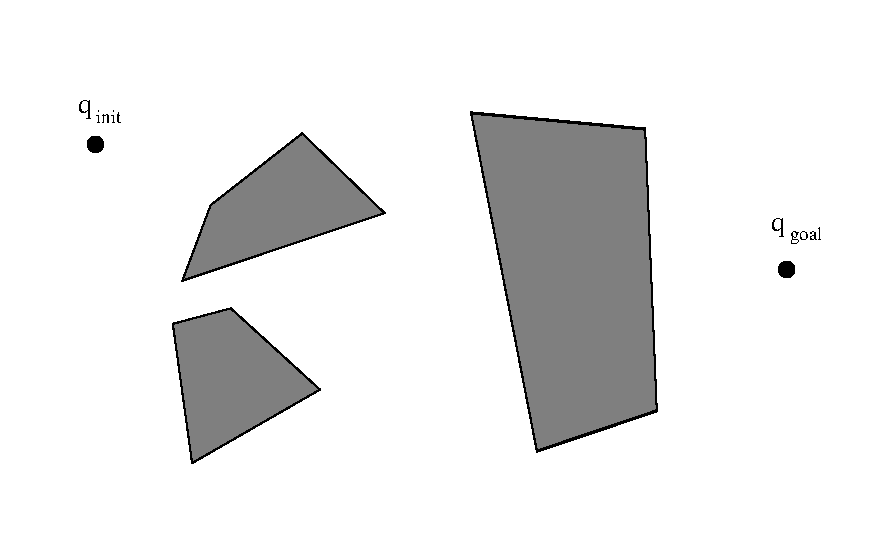
\includegraphics[width=.8\linewidth]{figures/RRT00.pdf}
}
\end{frame}

\begin{frame} {Rapidly exploring Random Tree (RRT) 2000}
\centerline {
  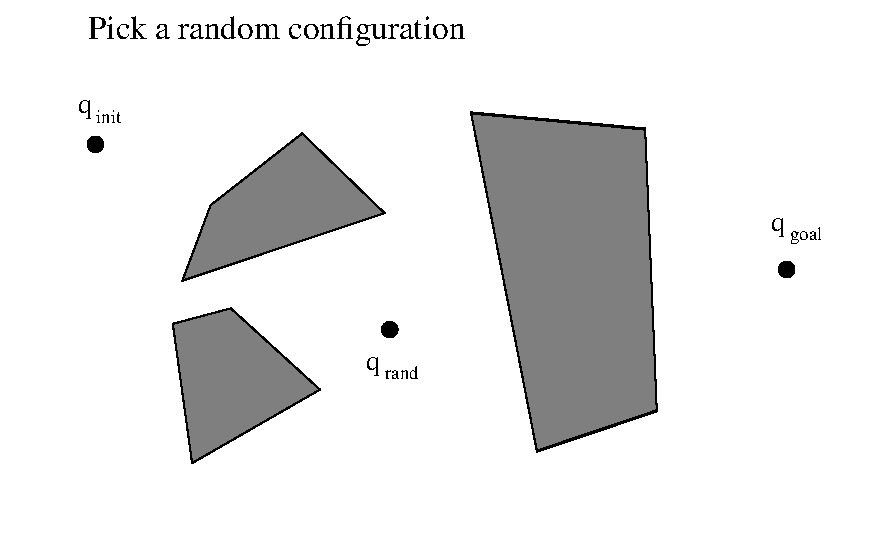
\includegraphics[width=.8\linewidth]{figures/RRT01.pdf}
}
\end{frame}

\begin{frame} {Rapidly exploring Random Tree (RRT) 2000}
\centerline {
  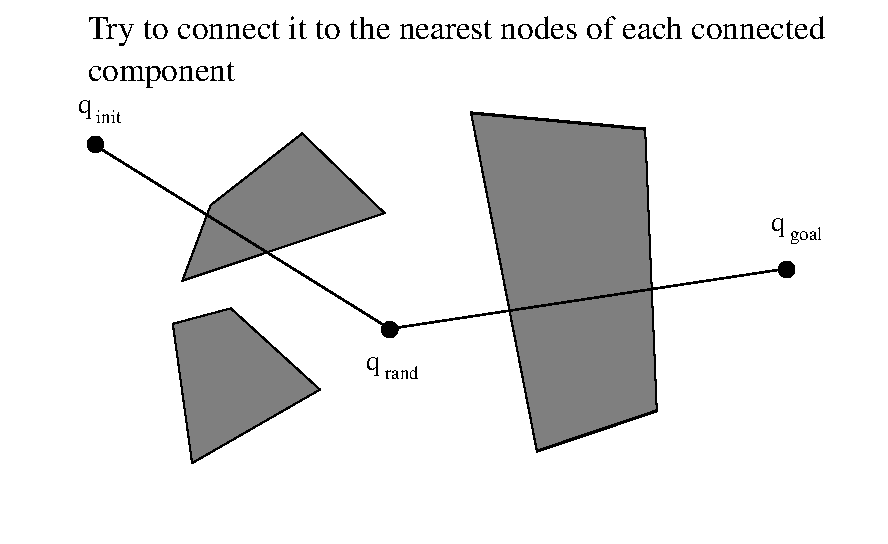
\includegraphics[width=.8\linewidth]{figures/RRT02.pdf}
}
\end{frame}

\begin{frame} {Rapidly exploring Random Tree (RRT) 2000}
\centerline {
  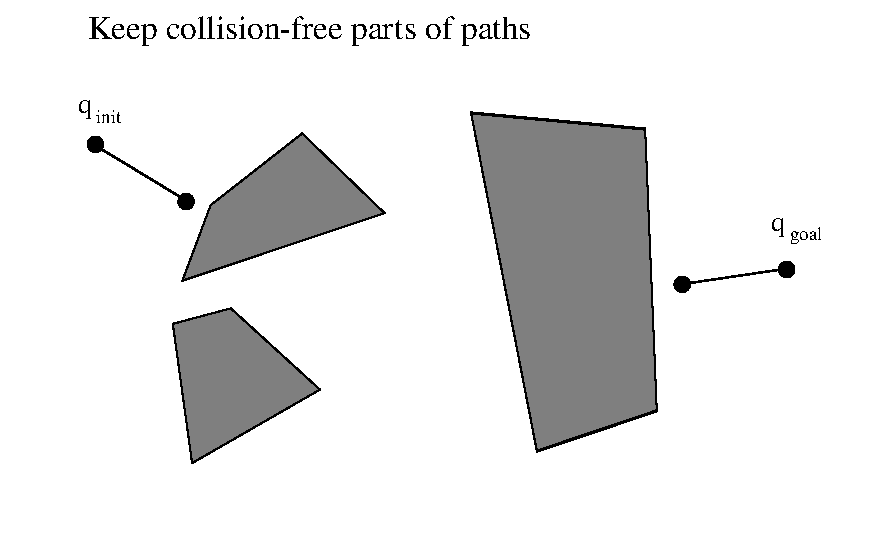
\includegraphics[width=.8\linewidth]{figures/RRT04.pdf}
}
\end{frame}

\begin{frame} {Rapidly exploring Random Tree (RRT) 2000}
\centerline {
  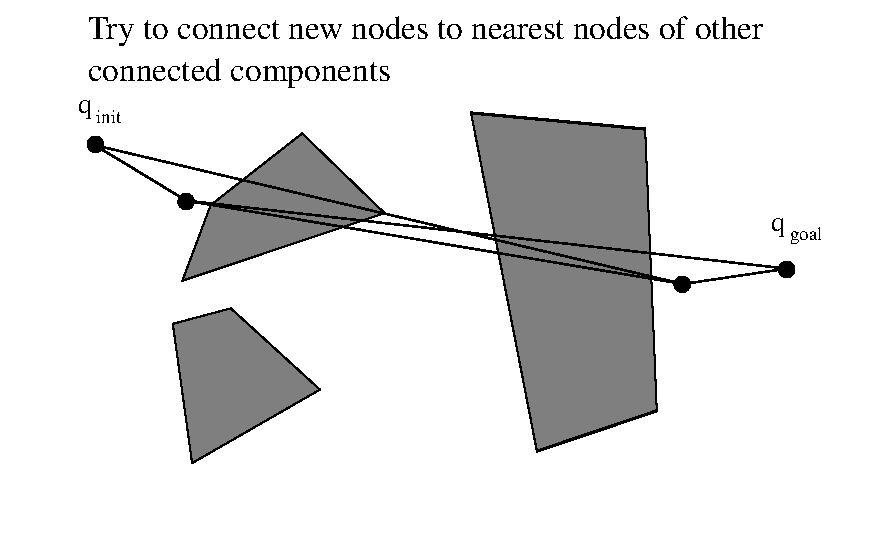
\includegraphics[width=.8\linewidth]{figures/RRT05.pdf}
}
\end{frame}

\begin{frame} {Rapidly exploring Random Tree (RRT) 2000}
\centerline {
  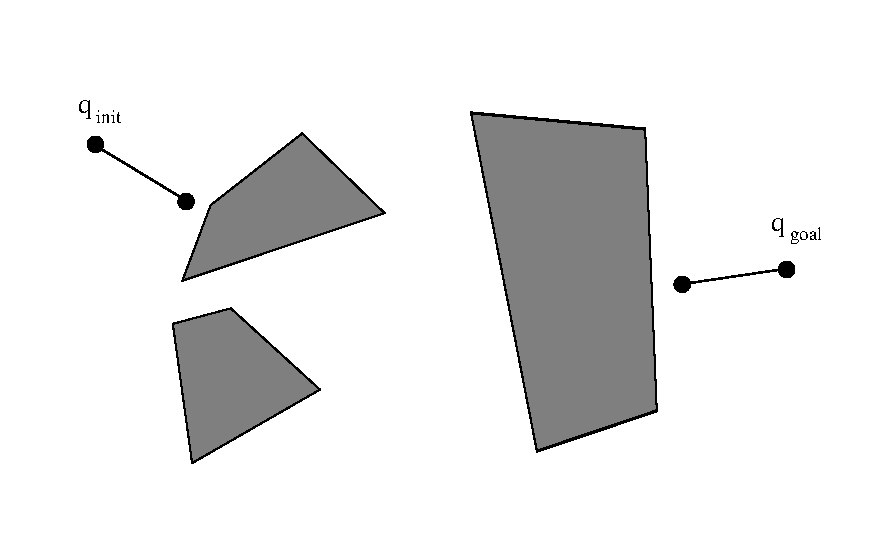
\includegraphics[width=.8\linewidth]{figures/RRT06.pdf}
}
\end{frame}

\begin{frame} {Rapidly exploring Random Tree (RRT) 2000}
\centerline {
  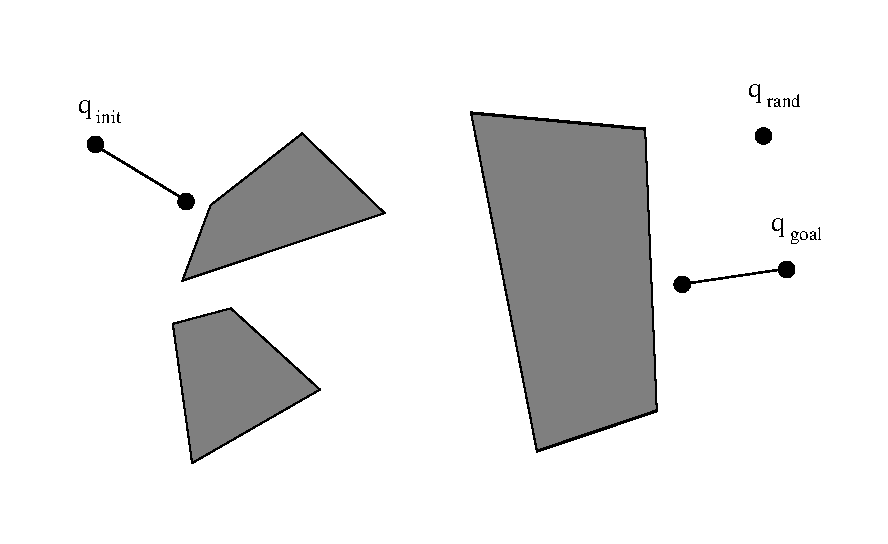
\includegraphics[width=.8\linewidth]{figures/RRT07.pdf}
}
\end{frame}

\begin{frame} {Rapidly exploring Random Tree (RRT) 2000}
\centerline {
  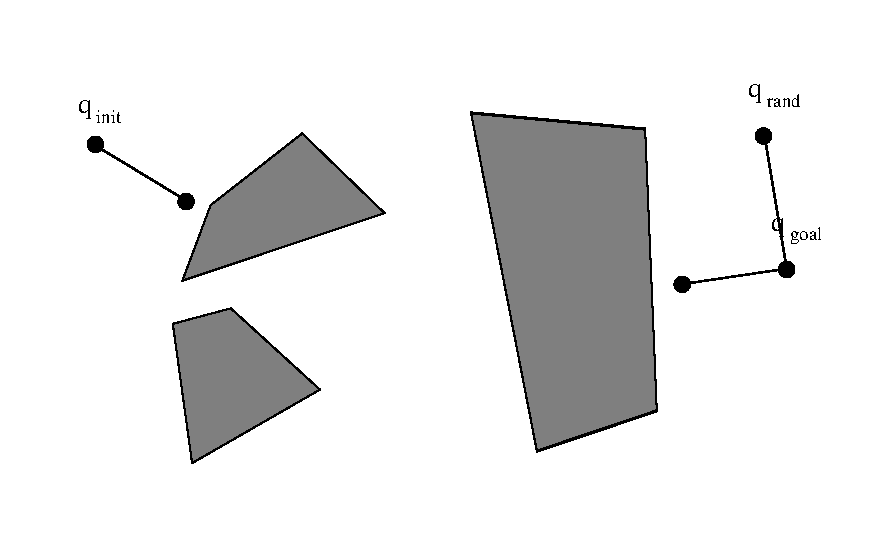
\includegraphics[width=.8\linewidth]{figures/RRT08.pdf}
}
\end{frame}

\begin{frame} {Rapidly exploring Random Tree (RRT) 2000}
\centerline {
  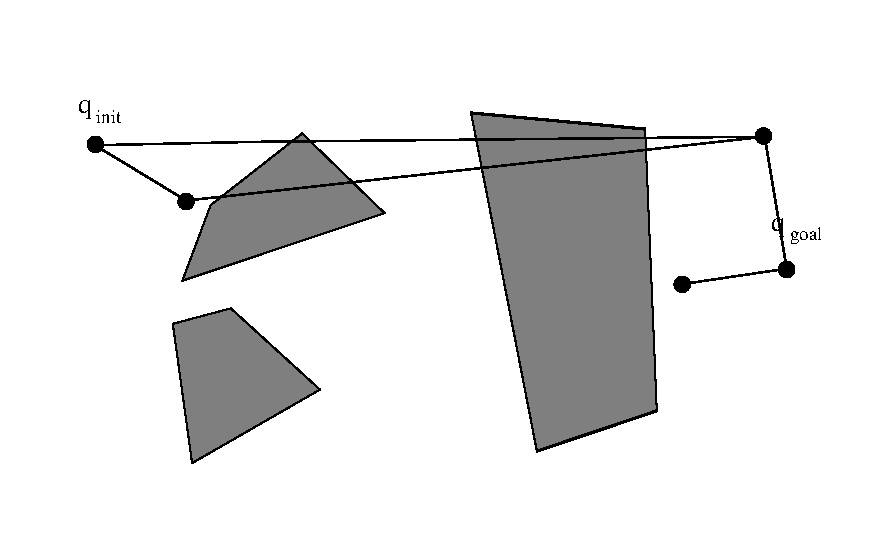
\includegraphics[width=.8\linewidth]{figures/RRT09.pdf}
}
\end{frame}

\begin{frame} {Rapidly exploring Random Tree (RRT) 2000}
\centerline {
  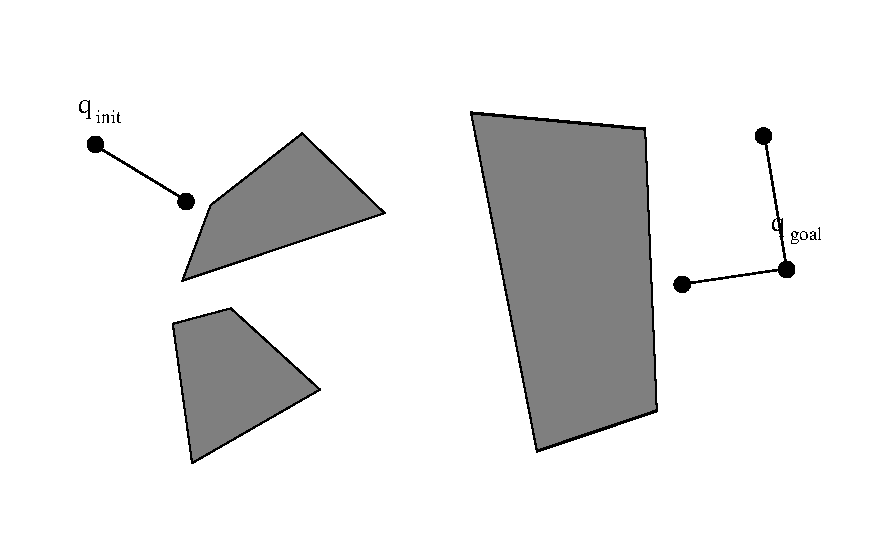
\includegraphics[width=.8\linewidth]{figures/RRT10.pdf}
}
\end{frame}

\begin{frame} {Rapidly exploring Random Tree (RRT) 2000}
\centerline {
  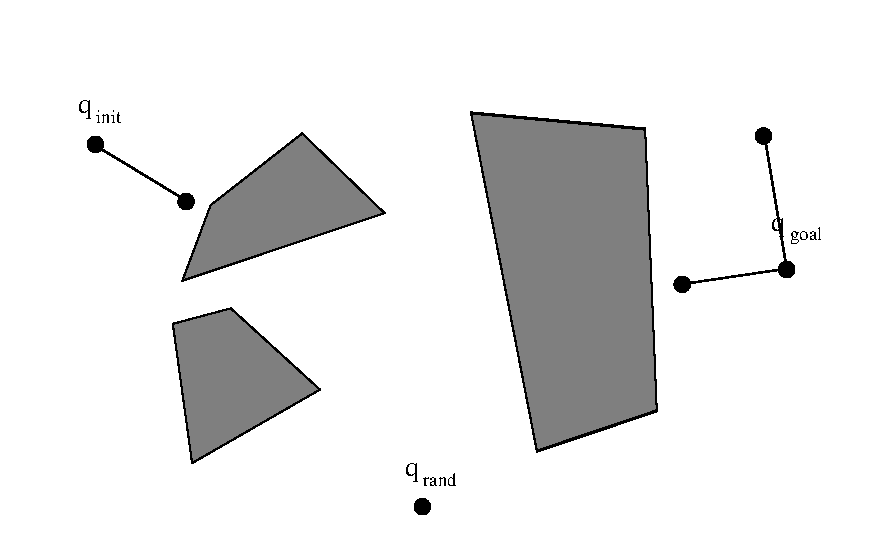
\includegraphics[width=.8\linewidth]{figures/RRT11.pdf}
}
\end{frame}

\begin{frame} {Rapidly exploring Random Tree (RRT) 2000}
\centerline {
  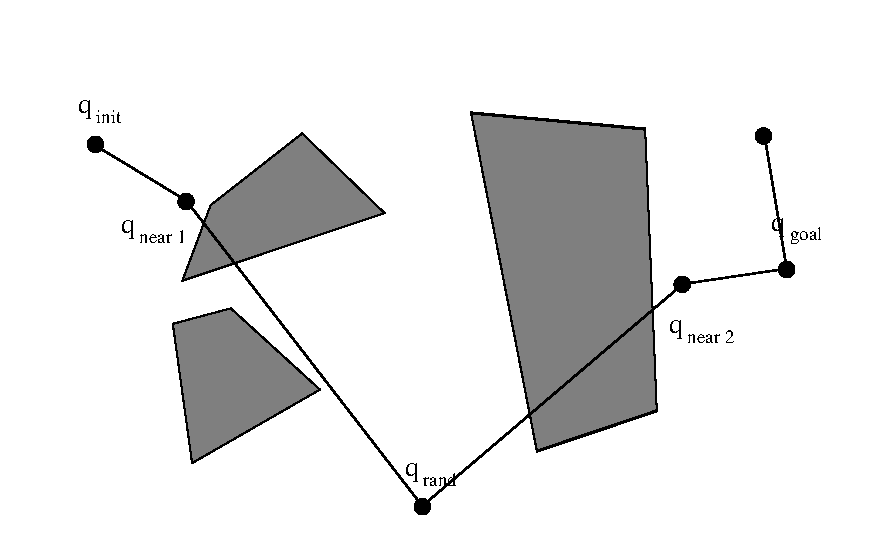
\includegraphics[width=.8\linewidth]{figures/RRT12.pdf}
}
\end{frame}

\begin{frame} {Rapidly exploring Random Tree (RRT) 2000}
\centerline {
  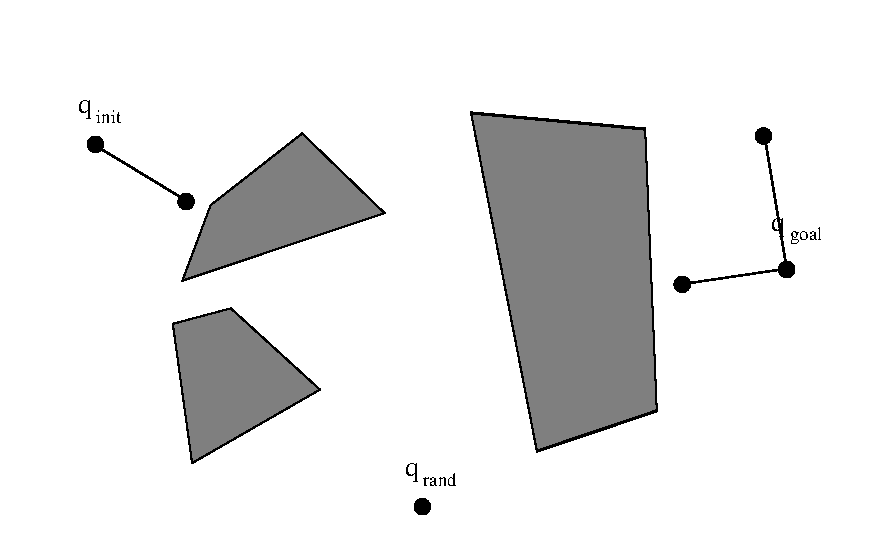
\includegraphics[width=.8\linewidth]{figures/RRT13.pdf}
}
\end{frame}

\begin{frame} {Rapidly exploring Random Tree (RRT) 2000}
\centerline {
  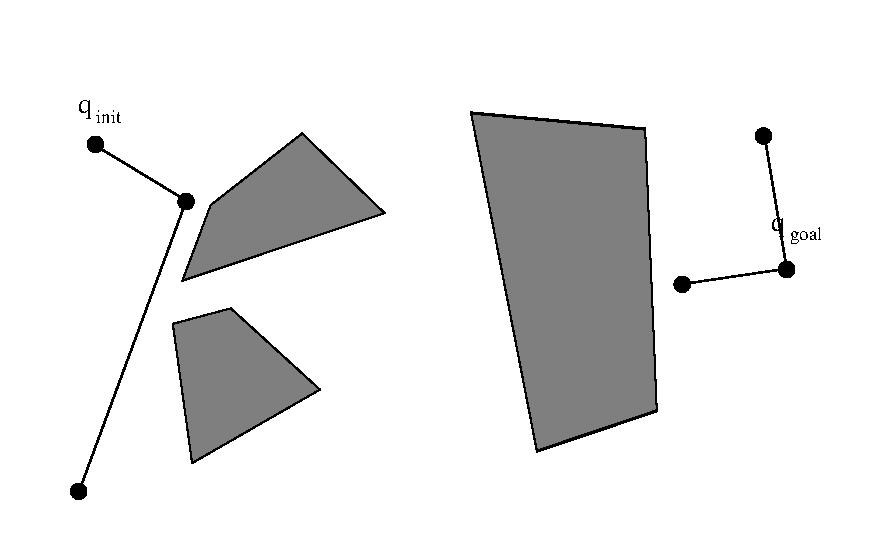
\includegraphics[width=.8\linewidth]{figures/RRT14.pdf}
}
\end{frame}

\begin{frame} {Rapidly exploring Random Tree (RRT) 2000}
\centerline {
  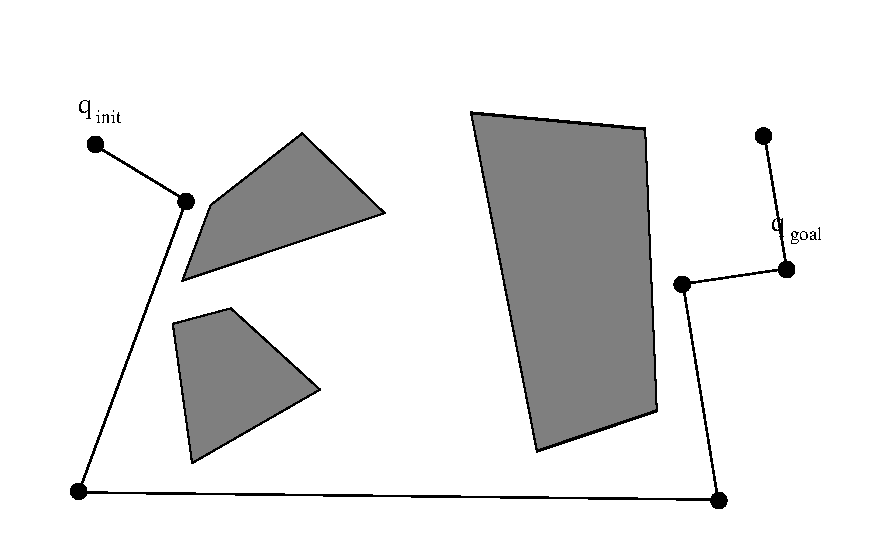
\includegraphics[width=.8\linewidth]{figures/RRT15.pdf}
}
\end{frame}

\begin{frame} {Rapidly exploring Random Tree (RRT) 2000}
\centerline {
  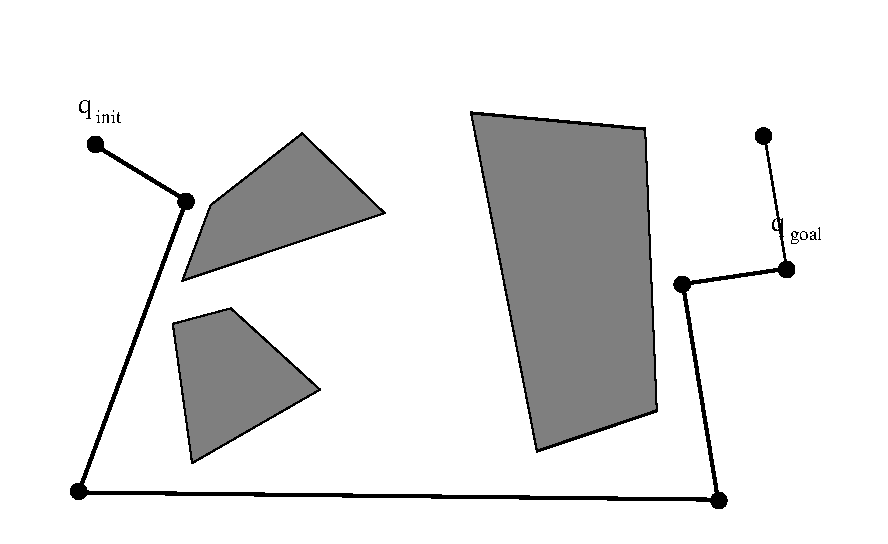
\includegraphics[width=.8\linewidth]{figures/RRT16.pdf}
}
\end{frame}

%
% random methods
%

\begin{frame} {Random methods}
  \begin{itemize}
  \item Pros:
    \begin{itemize}
    \item no explicit computation of the free configuration space,
    \item easy to implement,
    \item robust.
    \end{itemize}
    \pause
  \item Cons:
    \begin{itemize}
    \item no completeness property, only probabilistic completeness,
    \item difficult to find narrow passages.
    \end{itemize}
    \pause
  \item Requested operators~:
    \begin{itemize}
    \item Collision tests
      \begin{itemize}
      \item for configurations (static),
      \item for paths (dynamic)
      \end{itemize}
    \end{itemize}
  \end{itemize}
\end{frame}

%
% asymptotically optimal random sampling
%

\begin{frame} {Asymptotically optimal random methods}
  Asymptotically optimal variants of PRM and RRT exist:
  \begin{itemize}
  \item when the number of nodes tends to infinity,
  \item the solution computed by the algorithm tends to the optimal
    collision-free path.
  \end{itemize}
\end{frame}

%
%  PRM*
%

\begin{frame} {PRM*}
  \parbox{.49\linewidth} {
    \begin{algorithmic}
      \STATE \textbf{PRM}
      \STATE{$V\gets\emptyset$, $E\gets\emptyset$}
      \FOR{$i\in\{1,\cdots,n\}$}
      \STATE{$\conf_{rand}\gets$ {SampleFree}$_i$}
      \STATE{$U\gets G.near(\conf_{rand},r)$}
      \FORALL{$\conf\in U$ in order of increasing $\|\conf-\conf_{rand}\|$}
      \IF{$\conf_{rand}$ and $\conf$ in different connected components}
      \STATE{TryConnect($\conf_{rand},\conf$)}
      \ENDIF
      \ENDFOR
      \ENDFOR
    \end{algorithmic}
  }
  \pause
  \parbox{.49\linewidth} {
    \begin{algorithmic}
      \STATE \textbf{PRM*}
      \STATE{$V\gets$ {SampleFree}$_{i=1,\cdots,n}$, $E\gets\emptyset$}
      \FORALL{$\conf\in V$}
      \STATE{$U\gets G.near(\conf,{\color{red}r^{*}})\setminus\conf$}
      \FORALL{$\conf'\in U$}
      \STATE{TryConnect($\conf,\conf'$)}
      \ENDFOR
      \ENDFOR
    \end{algorithmic}
    {\color{red}$r^{*}$}=$\gamma_{PRM}(\log(n)/n)^{\frac{1}{d}}$
  }
\end{frame}

%
%  kPRM*
%

\begin{frame} {kPRM*}
  \parbox{.49\linewidth} {
    \begin{algorithmic}
      \STATE \textbf{kPRM}
      \STATE{$V\gets\emptyset$, $E\gets\emptyset$}
      \FOR{$i\in\{1,\cdots,n\}$}
      \STATE{$\conf_{rand}\gets$ {SampleFree}$_i$}
      \STATE{$U\gets G.nearest(\conf_{rand},k)$}
      \FORALL{$\conf\in U$ in order of increasing $\|\conf-\conf_{rand}\|$}
      \IF{$\conf_{rand}$ and $\conf$ in different connected components}
      \STATE{TryConnect($\conf_{rand},\conf$)}
      \ENDIF
      \ENDFOR
      \ENDFOR
    \end{algorithmic}
  }
  \pause
  \parbox{.49\linewidth} {
    \begin{algorithmic}
      \STATE \textbf{kPRM*}
      \STATE{$V\gets$ {SampleFree}$_{i=1,\cdots,n}$, $E\gets\emptyset$}
      \FORALL{$\conf\in V$}
      \STATE{$U\gets G.nearest(\conf,{\color{red}k^{*}})\setminus\conf$}
      \FORALL{$\conf'\in U$}
      \STATE{TryConnect($\conf,\conf'$)}
      \ENDFOR
      \ENDFOR
    \end{algorithmic}
    \begin{eqnarray*}
      {\color{red}k^{*}}&=&k_{PRM}(\log(n)),\\
      k_{PRM}&>&e(1+\frac{1}{d})
    \end{eqnarray*}
  }
\end{frame}

%
%  PRM*, kPRM*
%

\begin{frame} {PRM*,kPRM*}
  Note that
  \begin{itemize}
  \item PRM* and kPRM* are not iterative anymore,
  \item making them iterative is not trivial.
  \end{itemize}
\end{frame}

%
% RRT*, RMG
%

\begin{frame}
  There exists also asymptotically optimal variants of RRT
  \begin{itemize}
    \item RRG, RRT*
  \end{itemize}
  but they are specific to a given problem $(\conf_{init},\conf_{goal})$.
\end{frame}
